% !TeX program = pdflatex
% !TeX encoding = UTF-8
\documentclass[12pt,a4paper,oneside]{report}
% ============================================================================
% KONFIGURASI TEMPLATE — ubah nilai di file ini saja.
% ============================================================================

% Pilihan jenjang yang valid: sarjana atau magister
\def\jenjang{sarjana}
\def\jenjangSarjana{sarjana}
\def\jenjangMagister{magister}
\newif\ifmagister
\ifx\jenjang\jenjangMagister
  \magistertrue
\else\ifx\jenjang\jenjangSarjana
  \magisterfalse
\else
  \PackageError{UII-Template}{Jenjang '\jenjang' tidak dikenali}{Gunakan nilai 'sarjana' atau 'magister' pada config.tex.}
\fi\fi

% Data karya ilmiah
\newcommand{\judulTA}{BAGIAN INI ADALAH BAGIAN JUDUL}
\newcommand{\subjudulTA}{TULIS SUBJUDUL DI SINI JIKA ADA}
\newcommand{\judulInggris}{ENGLISH THESIS TITLE}
\newcommand{\subjudulInggris}{ENGLISH SUBTITLE IF APPLICABLE}

% Data mahasiswa
\newcommand{\namaMahasiswa}{NAMA MAHASISWA}
\newcommand{\nimMahasiswa}{20523000}
\newcommand{\konsentrasiMagister}{NAMA KONSENTRASI}

% Data pembimbing. Kosongkan namaPembimbingDua jika hanya ada satu pembimbing.
\newcommand{\namaPembimbing}{Nama Dosen Pembimbing, S.T., M.Eng.}
\newcommand{\nipPembimbing}{NIK/NIP Pembimbing}
\newcommand{\namaPembimbingDua}{}
\newcommand{\nipPembimbingDua}{}

% Data penguji
\newcommand{\namaPengujiSatu}{Nama Dosen Penguji 1, S.T., M.Sc.}
\newcommand{\nipPengujiSatu}{NIK/NIP Penguji 1}
\newcommand{\namaPengujiDua}{Nama Dosen Penguji 2, S.T., M.Cs.}
\newcommand{\nipPengujiDua}{NIK/NIP Penguji 2}
\newcommand{\namaPengujiTiga}{Nama Dosen Penguji 3, S.T., M.Kom.}
\newcommand{\nipPengujiTiga}{NIK/NIP Penguji 3}

% Data program studi dan waktu
\newcommand{\ketuaProgramStudi}{Nama Ketua Program Studi, S.T., M.Sc.}
\newcommand{\nipKetuaProgramStudi}{NIK/NIP Ketua Program Studi}
\newcommand{\tanggalPengesahan}{Tanggal Bulan Tahun}
\newcommand{\bulanLulus}{Bulan}
\newcommand{\tahunLulus}{2026}
\newcommand{\kotaTerbit}{Yogyakarta}

% Kata kunci
\newcommand{\kataKunci}{kata kunci pertama, kata kunci kedua, kata kunci ketiga}
\newcommand{\keywords}{keyword one, keyword two, keyword three}

% Nilai turunan otomatis berdasarkan jenjang.
\ifmagister
  \newcommand{\jenisDokumen}{Tesis}
  \newcommand{\jenisDokumenKapital}{TESIS}
  \newcommand{\namaProgram}{PROGRAM MAGISTER}
  \newcommand{\namaProgramKalimat}{Program Studi Informatika Program Magister}
  \newcommand{\gelarTarget}{Magister Komputer}
  \newcommand{\singkatanGelar}{M.Kom.}
\else
  \newcommand{\jenisDokumen}{Tugas Akhir}
  \newcommand{\jenisDokumenKapital}{TUGAS AKHIR}
  \newcommand{\namaProgram}{PROGRAM SARJANA}
  \newcommand{\namaProgramKalimat}{Program Studi Informatika Program Sarjana}
  \newcommand{\gelarTarget}{Sarjana Komputer}
  \newcommand{\singkatanGelar}{S.Kom.}
\fi

\usepackage[utf8]{inputenc}
\usepackage[T1]{fontenc}					% Proper font encoding for Indonesian/Latin characters
\usepackage[bahasa,english]{babel}			% Bilingual: Indonesian (bahasa) + English
\usepackage{verbatim}						% To use \begin{comment} text to comment \end{comment} or inserting codes \begin{verbatim}
%\usepackage{minted}						    % Insert code programming inline
\usepackage{listings}
\usepackage{xcolor}
\usepackage[titles]{tocloft}
\usepackage{cite}							% To cite your references
\usepackage{graphicx}						% Provide features to customize graphics
\usepackage{draftwatermark}					% To add a watermark : default = DRAFT
\usepackage{setspace}						% Provide support for setting the spacing between lines
\usepackage{titlesec}						% To modify the seciton titles
\usepackage{nomencl}						% To create nomenclature list
\makenomenclature							% Activate the nomenclature
\usepackage{acronym}						% To create Acronyms list
\usepackage{booktabs}
\usepackage{footnote}
\usepackage{caption}						% To manipulate captions for Figures and Tables
\DeclareCaptionFont{white}{\color{white}}
\DeclareCaptionFormat{listing}{\colorbox{gray}{\parbox{\textwidth}{#3}}}
\captionsetup[lstlisting]{format=listing,labelfont={bf,white},textfont={bf,white}}
\captionsetup{font=large}
\usepackage{subfig}
\usepackage{floatrow}						% To add a note under captions of Tables and Figures
\floatsetup[table]{capposition=top,font=large}			% To force the Tables captions back on top
\usepackage[flushleft]{threeparttable}		% To create tables with three sections (title, table, note)
\usepackage{array}							% To handle tabular and array environments
\usepackage{chngcntr}	
\usepackage{multirow}	
\usepackage{amsmath}

% To manipulate counters for Figures and Tables
\usepackage{pdfpages}						% To Include PDFS
\counterwithout{equation}{chapter} 			% Remove the chapter number in equations numbering
% \counterwithin{equation}{chapter}  		% Add the chapter number if you prefer but I think it's not correct with given format
\counterwithin{table}{chapter} 			% Remove the chapter number in tables numbering
% set the default margins of the layout, it will be overwritten at the beginning for first pages
\usepackage[a4paper,top=25mm,bottom=25mm,left=20mm,right=20mm,bindingoffset=10mm]{geometry}
\pagestyle{plain}
% Redefinition of the chapter command
\makeatletter
\def\@chapter[#1]#2{\ifnum \c@secnumdepth >\m@ne
                       \if@mainmatter
                         \refstepcounter{chapter}%
                         \typeout{\@chapapp \space \thechapter.}%
                         \addcontentsline{toc}{chapter}%
                                   {\protect\numberline{\thechapter}#1}%
                       \else				
                         \addcontentsline{toc}{chapter}{#1}%
                       \fi
                    \else                      
                      \addcontentsline{toc}{chapter}{#1}%
                    \fi
                    \chaptermark{#1}%
                    \if@twocolumn
                      \@topnewpage[\@makechapterhead{#2}]%
                    \else
                      \@makechapterhead{#2}%
                      \@afterheading
                    \fi}
\makeatother

\titleformat{\chapter}[display]
{\fontsize{30}{10}\selectfont 
\normalfont\bfseries\centering}
{\fontsize{30}{10}\selectfont \chaptertitlename\ \thechapter}{0.5em}{}

\makeatletter \@removefromreset{figure}{chapter}\makeatother

%% Bilingual section headings (Indonesian primary)
\renewcommand{\contentsname}{Daftar Isi}
\renewcommand{\listfigurename}{Daftar Gambar}
\renewcommand{\listtablename}{Daftar Tabel}
\renewcommand{\bibname}{Daftar Pustaka}
\renewcommand{\appendixname}{Lampiran}
\renewcommand{\thechapter}{\Roman{chapter}}
\renewcommand{\thesection}{\arabic{chapter}.\arabic{section}}

\titleformat{\section}{\normalfont\Large\bfseries}{\thesection}{1em}{\setstretch{0.1}}

\renewcommand{\emph}[1]{``#1''}
\renewcommand{\thefigure}{\arabic{chapter}.\arabic{figure}}
\renewcommand{\thetable}{\arabic{chapter}.\arabic{table}}

\newcommand\T{\rule{0pt}{2.6ex}}       % Top strut - used in Tables to add space on Top of the cell
\newcommand\B{\rule[-1.2ex]{0pt}{0pt}} % Bottom strut - used in Tables to add space on Bottom of the cell

\renewcommand*\cftchapnumwidth{3em}
\renewcommand{\cftchapdotsep}{\cftdotsep}% Chapters should use dots in ToC

%%%% Language switching short commands %%%%%%%%%%%%%%%%%%%%%%%
\newcommand{\IDon}{\begin{otherlanguage}{bahasa}} %% Opens Indonesian writing
\newcommand{\IDoff}{\end{otherlanguage}}           %% Closes Indonesian writing
\newcommand{\ENon}{\begin{otherlanguage}{english}} %% Opens English writing
\newcommand{\ENoff}{\end{otherlanguage}}           %% Closes English writing

\setpdfmetadata

\begin{document}

% Cover berbeda menurut jenjang.
\ifmagister
  % Cover Tesis Program Magister.
\begin{titlepage}
  \thispagestyle{empty}
  \centering

  
\includegraphics[width=42mm]{uii-logo.png}

  \vspace{18mm}
  {\bfseries\fontsize{16}{24}\selectfont \cetakJudulIndonesia\par}

  \vspace{22mm}
  {\namaMahasiswa\par}
  {\nimMahasiswa\par}

  \vfill
  Tesis diajukan sebagai syarat untuk meraih gelar \gelarTarget\par
  Konsentrasi \konsentrasiMagister\par
  \namaProgramKalimat\par
  Fakultas Teknologi Industri\par
  Universitas Islam Indonesia\par
  \tahunLulus\par
\end{titlepage}

\else
  % Halaman judul mengikuti susunan Template Skripsi Informatika UII 2020.
\begin{titlepage}
  \thispagestyle{empty}
  \centering

  {\bfseries\fontsize{16}{24}\selectfont \cetakJudulIndonesia\par}

  % Pada template Word terdapat ruang kosong untuk teks tersembunyi
  % "HALAMAN JUDUL"; tidak ada teks "TUGAS AKHIR" yang terlihat.
  \vspace{28mm}
  
\includegraphics[width=52mm]{uii-logo.png}

  \vspace{10mm}
  {\fontsize{12}{18}\selectfont Disusun Oleh:\par}
  \vspace{12mm}
  \begin{tabular}{@{}p{28mm}p{5mm}p{65mm}@{}}
    N\,a\,m\,a & {\pemisahidentitas} & {\namaMahasiswa} \\
    NIM & {\pemisahidentitas} & {\nimMahasiswa} \\
  \end{tabular}

  \vfill
  {\bfseries\fontsize{12}{18}\selectfont
    PROGRAM STUDI INFORMATIKA \textendash{} \namaProgram\par
    FAKULTAS TEKNOLOGI INDUSTRI\par
    UNIVERSITAS ISLAM INDONESIA\par
    \tahunLulus\par
  }
\end{titlepage}

\fi

% Nomor awal berbeda: Magister mulai i, Sarjana mulai ii.
\clearpage
\pagenumbering{roman}
\ifmagister\setcounter{page}{1}\else\setcounter{page}{2}\fi
\pagestyle{fancy}

% Urutan front matter khusus jenjang.
\ifmagister
  \bagianawal{Lembar Pengesahan Pembimbing}

\noindent\AddToShipoutPictureBG*{%
  \put(\LenToUnit{60mm},\LenToUnit{87mm}){
\includegraphics[width=90mm]{UII-Watermark.png}}%
}

\begin{center}
  {\bfseries \cetakJudulIndonesia\par}
  \vspace{14mm}
  \namaMahasiswa\par
  \nimMahasiswa\par
  \vspace{18mm}
  \kotaTerbit, \tanggalPengesahan\par
\end{center}

\vfill
{\small\itshape Jika terdapat dua pembimbing yang telah bergelar doktor, pembimbing pertama diletakkan di sebelah kiri dan pembimbing kedua di sebelah kanan. Pembimbing yang belum bergelar doktor tidak perlu ditulis pada halaman ini.\par}

\vspace{8mm}
\ifdefempty{\namaPembimbingDua}{%
  \begin{center}
    Pembimbing\par
    \vspace{24mm}
    \namaPembimbing\par
  \end{center}\par
}{%
  \noindent\begin{tabularx}{\textwidth}{C C}
    Pembimbing I & Pembimbing II \\
    \addlinespace[24mm]
    \namaPembimbing & \namaPembimbingDua \\
  \end{tabularx}\par
}\par

  \bagianawal{Lembar Pengesahan Penguji}

\noindent\AddToShipoutPictureBG*{%
  \put(\LenToUnit{60mm},\LenToUnit{87mm}){
\includegraphics[width=90mm]{UII-Watermark.png}}%
}

\begin{center}
  {\bfseries \cetakJudulIndonesia\par}
  \vspace{12mm}
  \namaMahasiswa\par
  \nimMahasiswa\par
  \vspace{14mm}
  \kotaTerbit, \tanggalPengesahan\par
\end{center}

\vspace{8mm}
\noindent Tim Penguji,

\vspace{4mm}
\noindent\begin{tabularx}{\dimexpr\textwidth-\parindent\relax}{@{}Y C@{}}
  \namaPengujiSatu & \rule{40mm}{0.4pt} \\
  Ketua & \\
  \addlinespace[6mm]
  \namaPengujiDua & \rule{40mm}{0.4pt} \\
  Anggota I & \\
  \addlinespace[6mm]
  \namaPengujiTiga & \rule{40mm}{0.4pt} \\
  Anggota II & \\
\end{tabularx}\par

\vfill
{\centering\noindent
  Mengetahui,\par
  Ketua Program Studi Informatika Program Magister\par
  Fakultas Teknologi Industri\par
  Universitas Islam Indonesia\par
  \vspace{20mm}
  \ketuaProgramStudi\par
}

  \bagianawal{Abstrak}

\begin{center}
  {\bfseries \cetakJudulIndonesia}
\end{center}

\petunjuk{Abstrak merupakan ringkasan tesis yang berisi latar belakang, rumusan masalah, metode penelitian, temuan pokok, dan kesimpulan. Jumlah kata yang diperkenankan antara 300 hingga 800 kata.}

Tuliskan abstrak tesis dalam Bahasa Indonesia di sini. Teks abstrak harus dapat dibaca secara mandiri tanpa tabel, gambar, atau sitasi yang tidak dijelaskan.

\vspace{6mm}
\noindent\textbf{Kata kunci}\par
\noindent \kataKunci

  \bagianawal{Abstract}

\begin{center}
  {\bfseries \cetakJudulInggris}
\end{center}

\petunjuk{The English abstract must outline the main approach and findings of the thesis and contain between 300 and 800 words.}

Write the English abstract here. It should be a faithful English version of the Indonesian abstract and should be understandable without unexplained tables, figures, or citations.

\vspace{6mm}
\noindent\textbf{Keywords}\par
\noindent \keywords

  \bagianawal{Pernyataan Keaslian Tulisan}

Dengan ini saya menyatakan bahwa tesis ini merupakan tulisan asli dari penulis dan tidak berisi material yang telah diterbitkan sebelumnya atau tulisan dari penulis lain, terkecuali referensi atas material tersebut telah disebutkan dalam tesis. Apabila terdapat kontribusi penulis lain, nama penulis tersebut secara eksplisit telah disebutkan dalam tesis ini.

Dengan ini saya juga menyatakan bahwa segala kontribusi dari pihak lain terhadap tesis ini, termasuk bantuan analisis statistik, desain survei, analisis data, prosedur teknis yang bersifat signifikan, dan segala bentuk aktivitas penelitian yang dipergunakan atau dilaporkan dalam tesis ini telah secara eksplisit disebutkan dalam tesis.

Segala bentuk hak cipta yang terdapat dalam material dokumen tesis ini berada dalam kepemilikan pemilik hak cipta masing-masing. Apabila dibutuhkan, penulis telah mendapatkan izin dari pemilik hak cipta untuk menggunakan ulang materialnya dalam tesis ini.

\vfill
\begin{flushleft}
  \kotaTerbit, \tanggalPengesahan\par
  \vspace{24mm}
  \namaMahasiswa
\end{flushleft}

  \bagianawal{Daftar Publikasi}

\petunjuk{Tuliskan seluruh publikasi selama masa studi dengan format referensi APA. Kelompokkan berdasarkan jenis publikasi, misalnya jurnal, bab buku, prosiding konferensi, dan lain-lain.}

\begin{enumerate}
  \item Nama Penulis. (Tahun). Judul publikasi pertama. \textit{Nama Jurnal atau Prosiding}, volume(nomor), halaman.
  \item Nama Penulis. (Tahun). Judul publikasi kedua. \textit{Nama Jurnal atau Prosiding}, volume(nomor), halaman.
\end{enumerate}

\section*{Publikasi yang menjadi bagian dari tesis}

\petunjuk{Jika publikasi diikutsertakan dalam tesis, jelaskan bab tempat publikasi digunakan dan kontribusi setiap penulis. Jika tidak ada, tuliskan “Tidak ada publikasi yang menjadi bagian dari tesis”.}

Publikasi berikut menjadi bagian dari BAB 3:

\noindent\begin{tabularx}{\textwidth}{|Y|Y|}
  \hline
  \textbf{Kontributor} & \textbf{Jenis Kontribusi} \\
  \hline
  \namaMahasiswa{} (Anda) & Mendesain eksperimen dan menulis publikasi. \\
  \hline
  Nama Penulis Kedua & Berkontribusi pada desain eksperimen dan penyuntingan. \\
  \hline
  Nama Penulis Ketiga & Melakukan analisis statistik terhadap data penelitian. \\
  \hline
\end{tabularx}

\vspace{6mm}
\noindent Jika tidak ada publikasi yang disertakan dalam tesis, ganti seluruh contoh di atas dengan pernyataan: \textbf{Tidak ada publikasi yang menjadi bagian dari tesis.}

  \bagianawal{Halaman Kontribusi}

\petunjuk{Tuliskan kontribusi signifikan dari pihak lain dalam bentuk paragraf, bukan daftar. Kontribusi dapat meliputi konsep dan desain penelitian, analisis dan interpretasi data, penyusunan draf, atau perbaikan substansial yang mengubah interpretasi hasil penelitian.}

Tuliskan kontribusi pihak lain yang bersifat signifikan dan substansial di sini. Sebutkan nama kontributor serta bentuk kontribusinya secara jelas. Jika tidak ada kontribusi signifikan dari pihak lain, tuliskan: \textbf{Tidak ada kontribusi dari pihak lain.}

  \bagianawal{Halaman Persembahan}

\petunjuk{Halaman ini digunakan untuk menyampaikan terima kasih kepada pihak yang membantu secara akademik, non-akademik, atau finansial selama studi di Program Studi Informatika Program Magister.}

Tuliskan persembahan atau ucapan terima kasih di sini sebagai paragraf biasa yang dimulai dari bagian kiri atas area penulisan.

  \bagianawal{Kata Pengantar}

Puji syukur penulis panjatkan kepada Tuhan Yang Maha Esa karena \jenisDokumen{} ini dapat diselesaikan. Dokumen ini disusun sebagai salah satu syarat untuk memperoleh gelar \gelarTarget{} pada \namaProgramKalimat, Fakultas Teknologi Industri, Universitas Islam Indonesia.

Penulis menyampaikan terima kasih kepada dosen pembimbing, dosen penguji, keluarga, rekan, serta seluruh pihak yang telah memberikan arahan dan dukungan selama penyusunan \jenisDokumen{} ini. Penulis menyadari bahwa dokumen ini masih memiliki keterbatasan sehingga kritik dan saran yang membangun sangat diharapkan.

Semoga \jenisDokumen{} ini dapat memberikan manfaat bagi pembaca dan pengembangan ilmu pengetahuan di bidang Informatika.

\vfill
\begin{flushright}
  \kotaTerbit, \bulanLulus\ \tahunLulus\par
  \vspace{18mm}
  \namaMahasiswa
\end{flushright}

  \clearpage
\phantomsection
\addcontentsline{toc}{chapter}{\contentsname}
\begingroup
\singlespacing
\tableofcontents
\endgroup

  \clearpage
\phantomsection
\addcontentsline{toc}{chapter}{\listtablename}
\begingroup
\singlespacing
\listoftables
\endgroup

  \clearpage
\phantomsection
\addcontentsline{toc}{chapter}{\listfigurename}
\begingroup
\singlespacing
\listoffigures
\endgroup

  \bagianawal{Glosarium}

\petunjuk{Bagian ini opsional. Urutkan istilah secara alfabetis dan hapus istilah contoh yang tidak digunakan.}

\begin{description}[style=multiline,leftmargin=35mm,font=\normalfont]
  \item[Compile] Proses menerjemahkan berkas kode sumber dan berkas terkait menjadi bentuk yang dapat dijalankan atau diproses lebih lanjut.
  \item[Debug] Kegiatan menelusuri dan memperbaiki kesalahan pada perangkat lunak.
  \item[Waterfall] Salah satu model pengembangan perangkat lunak yang membagi proses ke dalam tahapan berurutan.
\end{description}

\else
  \bagianawaltanpatoc{HALAMAN PENGESAHAN DOSEN PEMBIMBING}

% Watermark kuning ditempatkan tepat di tengah halaman seperti template Word.
\AddToShipoutPictureBG*{%
  \put(\LenToUnit{60mm},\LenToUnit{87mm}){%
    
\includegraphics[width=90mm]{UII-Watermark.png}%
  }%
}

\begin{center}
  {\bfseries\fontsize{16}{24}\selectfont \cetakJudulIndonesia\par}
  \vspace{4mm}
  {\bfseries TUGAS AKHIR\par}
  \vspace{42mm}
  Disusun Oleh:\par
  \vspace{16mm}
  \begin{tabular}{@{}p{28mm}p{5mm}p{65mm}@{}}
    N\,a\,m\,a & {\pemisahidentitas} & {\namaMahasiswa} \\
    NIM & {\pemisahidentitas} & {\nimMahasiswa} \\
  \end{tabular}
\end{center}

\vspace{38mm}
\begin{center}
  \kotaTerbit, \tanggalPengesahan\par
  Pembimbing,\par
  \vspace{25mm}
  \namaPembimbing
\end{center}

  \bagianawaltanpatoc{HALAMAN PENGESAHAN DOSEN PENGUJI}

\begin{center}
  {\bfseries\fontsize{16}{24}\selectfont \cetakJudulIndonesia\par}
  \vspace{6mm}
  {\bfseries TUGAS AKHIR\par}
  \vspace{6mm}
  Telah dipertahankan di depan sidang penguji sebagai salah satu syarat untuk memperoleh gelar Sarjana Komputer dari Program Studi Informatika \textendash{} Program Sarjana, Fakultas Teknologi Industri, Universitas Islam Indonesia.\par
  \vspace{6mm}
  \kotaTerbit, \tanggalPengesahan
\end{center}

\vspace{8mm}
\noindent
\begin{tabularx}{\textwidth}{@{}Y C@{}}
  \textbf{Tim Penguji} & \\
  \addlinespace[2mm]
  \namaPengujiSatu & \rule{40mm}{0.4pt} \\
  \addlinespace[7mm]
  \textbf{Anggota 1} & \\
  \addlinespace[1mm]
  \namaPengujiDua & \rule{40mm}{0.4pt} \\
  \addlinespace[7mm]
  \textbf{Anggota 2} & \\
  \addlinespace[1mm]
  \namaPengujiTiga & \rule{40mm}{0.4pt} \\
\end{tabularx}

\vfill
\begin{center}
  Mengetahui,\par
  Ketua Program Studi Informatika \textendash{} Program Sarjana\par
  Fakultas Teknologi Industri\par
  Universitas Islam Indonesia\par
  \vspace{22mm}
  \ketuaProgramStudi
\end{center}

  \bagianawaltanpatoc{HALAMAN PERNYATAAN KEASLIAN TUGAS AKHIR}

\noindent Yang bertanda tangan di bawah ini:

\vspace{5mm}
\noindent
\begin{tabular}{@{}p{22mm}p{5mm}p{113mm}@{}}
  Nama & {\pemisahidentitas} & \namaMahasiswa \\
  NIM & {\pemisahidentitas} & \nimMahasiswa \\
\end{tabular}

\vspace{6mm}
\noindent Tugas akhir dengan judul:

\begin{center}
  \textbf{\cetakJudulIndonesia}
\end{center}

Menyatakan bahwa seluruh komponen dan isi dalam tugas akhir ini adalah hasil karya saya sendiri. Apabila di kemudian hari terbukti bahwa sebagian atau seluruh karya ini bukan hasil karya sendiri, saya bersedia menerima sanksi akademik sesuai dengan ketentuan yang berlaku di Universitas Islam Indonesia.

Demikian surat pernyataan ini dibuat dengan sebenar-benarnya agar dapat dipergunakan sebagaimana mestinya.

\vfill
\begin{flushright}
  \kotaTerbit, \tanggalPengesahan\par
  Yang menyatakan,\par
  \vspace{25mm}
  \namaMahasiswa
\end{flushright}

  \bagianawaltanpatoc{HALAMAN PERSEMBAHAN}

\petunjuk{Halaman ini opsional. Hapus kotak petunjuk dan isi dengan kalimat persembahan yang tidak melanggar etika. Idealnya bagian ini tidak lebih dari satu halaman.}

Tuliskan persembahan di sini sebagai paragraf biasa. Isi dimulai dari bagian kiri atas area penulisan, bukan dari tengah halaman.

  \bagianawaltanpatoc{HALAMAN MOTO}

\petunjuk{Halaman ini opsional. Tuliskan moto secara ringkas dan cantumkan sumber apabila mengutip pernyataan orang lain.}

\begin{center}
  \textit{``Tuliskan moto di sini.''}\par
  \vspace{4mm}
  --- Sumber moto
\end{center}

  \bagianawal{Kata Pengantar}

Puji syukur penulis panjatkan kepada Tuhan Yang Maha Esa karena \jenisDokumen{} ini dapat diselesaikan. Dokumen ini disusun sebagai salah satu syarat untuk memperoleh gelar \gelarTarget{} pada \namaProgramKalimat, Fakultas Teknologi Industri, Universitas Islam Indonesia.

Penulis menyampaikan terima kasih kepada dosen pembimbing, dosen penguji, keluarga, rekan, serta seluruh pihak yang telah memberikan arahan dan dukungan selama penyusunan \jenisDokumen{} ini. Penulis menyadari bahwa dokumen ini masih memiliki keterbatasan sehingga kritik dan saran yang membangun sangat diharapkan.

Semoga \jenisDokumen{} ini dapat memberikan manfaat bagi pembaca dan pengembangan ilmu pengetahuan di bidang Informatika.

\vfill
\begin{flushright}
  \kotaTerbit, \bulanLulus\ \tahunLulus\par
  \vspace{18mm}
  \namaMahasiswa
\end{flushright}

  \bagianawal{SARI}

\petunjuk{Ganti isi contoh berikut dengan ringkasan yang memuat latar belakang, tujuan atau masalah, metode, hasil utama, dan kesimpulan. Gunakan satu halaman dan tuliskan kata kunci di bagian akhir.}

Paragraf pertama menjelaskan latar belakang dan masalah utama yang melandasi pelaksanaan tugas akhir. Uraian harus singkat, mandiri, dan dapat dipahami tanpa harus membaca keseluruhan laporan.

Paragraf kedua menjelaskan metode, data, perangkat, atau tahapan yang digunakan untuk menyelesaikan masalah. Hindari sitasi, tabel, gambar, dan singkatan yang belum dijelaskan di dalam sari.

Paragraf ketiga menjelaskan hasil utama dan kesimpulan yang diperoleh. Cantumkan hasil kuantitatif penting apabila tersedia dan hindari pernyataan yang tidak didukung oleh hasil tugas akhir.

\vspace{6mm}
\noindent\textbf{Kata kunci:} \kataKunci.

  \bagianawal{Glosarium}

\petunjuk{Bagian ini opsional. Urutkan istilah secara alfabetis dan hapus istilah contoh yang tidak digunakan.}

\begin{description}[style=multiline,leftmargin=35mm,font=\normalfont]
  \item[Compile] Proses menerjemahkan berkas kode sumber dan berkas terkait menjadi bentuk yang dapat dijalankan atau diproses lebih lanjut.
  \item[Debug] Kegiatan menelusuri dan memperbaiki kesalahan pada perangkat lunak.
  \item[Waterfall] Salah satu model pengembangan perangkat lunak yang membagi proses ke dalam tahapan berurutan.
\end{description}

  \clearpage
\phantomsection
\addcontentsline{toc}{chapter}{\contentsname}
\begingroup
\singlespacing
\tableofcontents
\endgroup

  \clearpage
\phantomsection
\addcontentsline{toc}{chapter}{\listtablename}
\begingroup
\singlespacing
\listoftables
\endgroup

  \clearpage
\phantomsection
\addcontentsline{toc}{chapter}{\listfigurename}
\begingroup
\singlespacing
\listoffigures
\endgroup

\fi

% Bagian utama tetap shared pada tahap ini.
\clearpage
\pagenumbering{arabic}
\setcounter{page}{1}
\pagestyle{fancy}

\chapter{PENDAHULUAN}

\petunjuk{Gunakan bab ini untuk menjelaskan latar belakang, rumusan masalah, batasan masalah, tujuan, manfaat, metodologi singkat, dan sistematika penulisan. Hapus seluruh kotak petunjuk sebelum penyerahan akhir.}

\section{Latar Belakang}

Tuliskan latar belakang secara runtut dari konteks umum menuju masalah khusus yang akan diselesaikan. Setiap paragraf menggunakan Times New Roman 12 pt, spasi 1,5, rata kanan-kiri, dan indentasi baris pertama 1 cm. Hindari paragraf yang hanya terdiri dari satu kalimat.

\subsection{Contoh Anak Subbab}

Anak subbab menggunakan penomoran tiga tingkat, misalnya 1.1.1. Anak subbab dicetak tebal dan dimasukkan ke dalam Daftar Isi.

\subsubsection*{Contoh Cucu Subbab}

Cucu subbab dicetak tebal tanpa nomor. Cucu subbab tidak dimasukkan ke dalam Daftar Isi. Gunakan tingkat ini hanya bila uraian benar-benar memerlukan pembagian tambahan di bawah anak subbab.

\section{Rumusan Masalah}

Rumusan masalah harus konsisten dengan tujuan dan kesimpulan. Apabila perlu dituliskan sebagai daftar, gunakan format berikut.

\begin{enumerate}
  \item Bagaimana merancang solusi untuk permasalahan yang telah diidentifikasi?
  \item Bagaimana mengevaluasi solusi tersebut menggunakan ukuran yang relevan?
\end{enumerate}

\section{Batasan Masalah}

Batasan masalah menjelaskan ruang lingkup data, pengguna, teknologi, lokasi, waktu, atau fitur yang termasuk dan tidak termasuk dalam tugas akhir.

\section{Tujuan Penelitian}

Tujuan harus menjawab rumusan masalah dan menggunakan kata kerja yang dapat dievaluasi, misalnya merancang, mengimplementasikan, membandingkan, atau mengukur.

\section{Manfaat Penelitian}

Jelaskan manfaat akademik dan manfaat praktis yang diharapkan dari hasil tugas akhir.

\section{Sistematika Penulisan}

Jelaskan isi setiap bab secara singkat agar pembaca memahami alur keseluruhan laporan.

I have an apple, I have a pen...

Citation example, deep learning \cite{lecun2015deep} is ...

\section{Apple}

Figure \ref{fig:ch2_apple} shows an apple.

\begin{figure}[!ht]
    \centering
    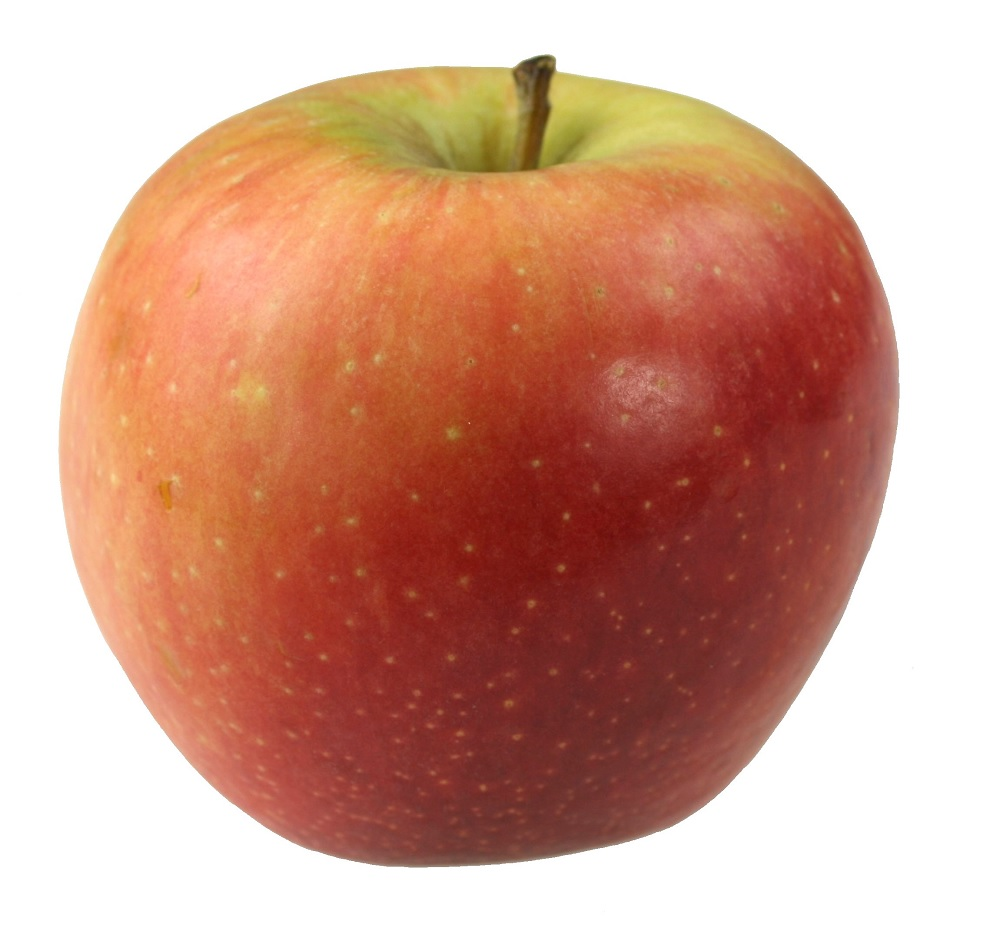
\includegraphics[width=0.3\linewidth]{Images/chapter2/apple.jpg}
    \caption[Apple]{Apple.}
    \label{fig:ch2_apple}
\end{figure}

Table \ref{tab:ch2_fruit_price} shows the apple price.

\begin{table}[ht]
\centering
\caption{Fruit Price}
\label{tab:ch2_fruit_price}
\begin{tabular}{|l|l|}
\hline
\textbf{Fruit Name} & \textbf{Price} \\ \hline
Apple               & 10             \\ \hline
\end{tabular}
\end{table}

Bigger table below

\begin{table}[ht]
\centering
\caption{Fruit Price}
\label{tab:ch2_fruit_price}
\resizebox{\columnwidth}{!}{
\begin{tabular}{|l|l|}
\hline
\textbf{Fruit Name} & \textbf{Price} \\ \hline
Apple               & 10             \\ \hline
\end{tabular}}
\end{table}
\chapter{METODOLOGI PENELITIAN}

\petunjuk{Jelaskan objek penelitian, data, alat, tahapan, metode pengumpulan data, metode analisis, serta cara pengujian. Bab ini juga memuat contoh persamaan dan kode program.}

\section{Tahapan Penelitian}

Tahapan penelitian harus disajikan secara berurutan dan dapat direplikasi. Contoh tahapan umum adalah identifikasi masalah, pengumpulan data, perancangan solusi, implementasi, pengujian, dan evaluasi.

\section{Contoh Persamaan}

Sebelum persamaan ditampilkan, jelaskan variabel dan tujuan penggunaannya. Nilai rata-rata dapat dihitung menggunakan Persamaan~\eqref{eq:rata-rata}.

\begin{equation}
  \bar{x} = \frac{1}{n}\sum_{i=1}^{n}x_i
  \label{eq:rata-rata}
\end{equation}

Pada Persamaan~\eqref{eq:rata-rata}, $\bar{x}$ adalah nilai rata-rata, $x_i$ adalah nilai pengamatan ke-$i$, dan $n$ adalah jumlah pengamatan. Nomor persamaan dibuat otomatis berdasarkan nomor bab.

\section{Contoh Kode Program}

Notasi algoritmik, kode program, atau pseudocode menggunakan font monospaced 9 pt dan spasi tunggal. Kode yang panjang sebaiknya ditempatkan di lampiran, sedangkan bagian inti hanya menampilkan potongan yang dibahas. Contoh ditunjukkan pada Gambar~\ref{fig:contoh-kode}.

\begin{figure}[H]
\begin{minipage}{\textwidth}
\begin{lstlisting}[language=Python]
def hitung_rata_rata(data):
    if not data:
        return 0
    return sum(data) / len(data)
\end{lstlisting}
\end{minipage}
\caption{Contoh kode program untuk menghitung nilai rata-rata}
\label{fig:contoh-kode}
\end{figure}

\section{Metode Pengujian}

Jelaskan skenario, data uji, metrik, kriteria keberhasilan, dan cara interpretasi hasil. Setiap klaim pada bab hasil harus dapat ditelusuri kembali ke metode yang dijelaskan pada bagian ini.

\chapter{HASIL DAN PEMBAHASAN}

\petunjuk{Pisahkan penyajian hasil dari interpretasinya. Setiap tabel, gambar, dan nilai numerik harus dijelaskan dalam narasi serta dihubungkan dengan tujuan dan kajian pustaka.}

\section{Hasil Implementasi}

Jelaskan hasil implementasi dengan urutan yang konsisten terhadap tahapan metodologi. Gunakan tangkapan layar hanya jika elemen antarmuka perlu dibahas. Pastikan teks di dalam gambar tetap terbaca.

\section{Hasil Pengujian}

Tabel~\ref{tab:hasil-pengujian} menunjukkan contoh penyajian hasil beberapa skenario. Angka pada tabel ini hanya merupakan data contoh dan wajib diganti dengan hasil pengujian yang sebenarnya.

\begin{table}[H]
  \centering
  \caption{Contoh hasil pengujian sistem}
  \label{tab:hasil-pengujian}
  \begin{tabularx}{\textwidth}{YCC}
    \toprule
    \textbf{Skenario} & \textbf{Hasil yang Diharapkan} & \textbf{Status} \\
    \midrule
    Pengguna memasukkan data valid & Data tersimpan & Berhasil \\
    Pengguna memasukkan data kosong & Validasi ditampilkan & Berhasil \\
    Pengguna meminta laporan & Laporan dihasilkan & Berhasil \\
    \bottomrule
  \end{tabularx}
\end{table}

\section{Pembahasan}

Pembahasan tidak hanya mengulang angka hasil pengujian. Jelaskan penyebab hasil, keterkaitannya dengan teori atau penelitian sebelumnya, implikasi praktis, serta kondisi yang membatasi generalisasi hasil.

Ketika membandingkan hasil dengan penelitian lain, gunakan sitasi dari database referensi. Sebagai contoh, konsep penyusunan dokumen teknis terstruktur dapat dirujuk melalui \cite{lamport1994}.

\chapter{EVALUASI}

\petunjuk{Judul bab ini dapat disesuaikan dengan karakter tugas akhir. Jika evaluasi telah digabungkan dalam BAB IV, bab ini dapat diubah menjadi bab lain yang relevan atau dihapus dengan tetap menyesuaikan penomoran.}

\section{Evaluasi terhadap Tujuan}

Evaluasi menjelaskan sejauh mana setiap tujuan penelitian telah dicapai. Gunakan indikator yang telah didefinisikan pada metodologi dan hindari memperkenalkan metrik baru tanpa penjelasan.

\section{Keterbatasan}

Tuliskan keterbatasan data, metode, perangkat, ruang lingkup, dan proses pengujian secara jujur. Keterbatasan bukan sekadar daftar kekurangan, tetapi menjadi dasar untuk memahami ruang berlaku hasil penelitian.

\section{Implikasi}

Jelaskan implikasi hasil bagi pengguna, organisasi, pengembang, atau penelitian lanjutan sesuai dengan konteks tugas akhir.

\chapter{KESIMPULAN DAN SARAN}

\petunjuk{Kesimpulan harus menjawab rumusan masalah dan tidak memuat hasil baru. Saran diturunkan dari keterbatasan atau peluang pengembangan yang ditemukan.}

\section{Kesimpulan}

Tuliskan kesimpulan secara ringkas berdasarkan hasil dan pembahasan. Pastikan setiap butir rumusan masalah pada BAB I memperoleh jawaban yang jelas dan didukung oleh hasil tugas akhir.

\section{Saran}

Tuliskan saran yang spesifik dan dapat ditindaklanjuti. Hindari saran yang terlalu umum, misalnya hanya menyatakan bahwa sistem perlu dikembangkan lebih lanjut tanpa menjelaskan bagian dan tujuan pengembangannya.


\clearpage
\ifmagister\def\bibname{Daftar Pustaka}\else\def\bibname{DAFTAR PUSTAKA}\fi
\phantomsection
\addcontentsline{toc}{chapter}{\bibname}
\bibliographystyle{apacite}
\bibliography{Bibliographies/references}

\paragraph{Sample PDF Complete} A simple inclusion of a PDF file. It will start on next page and be inserted. 
% Format command : \includepdf[page=-]{filename}
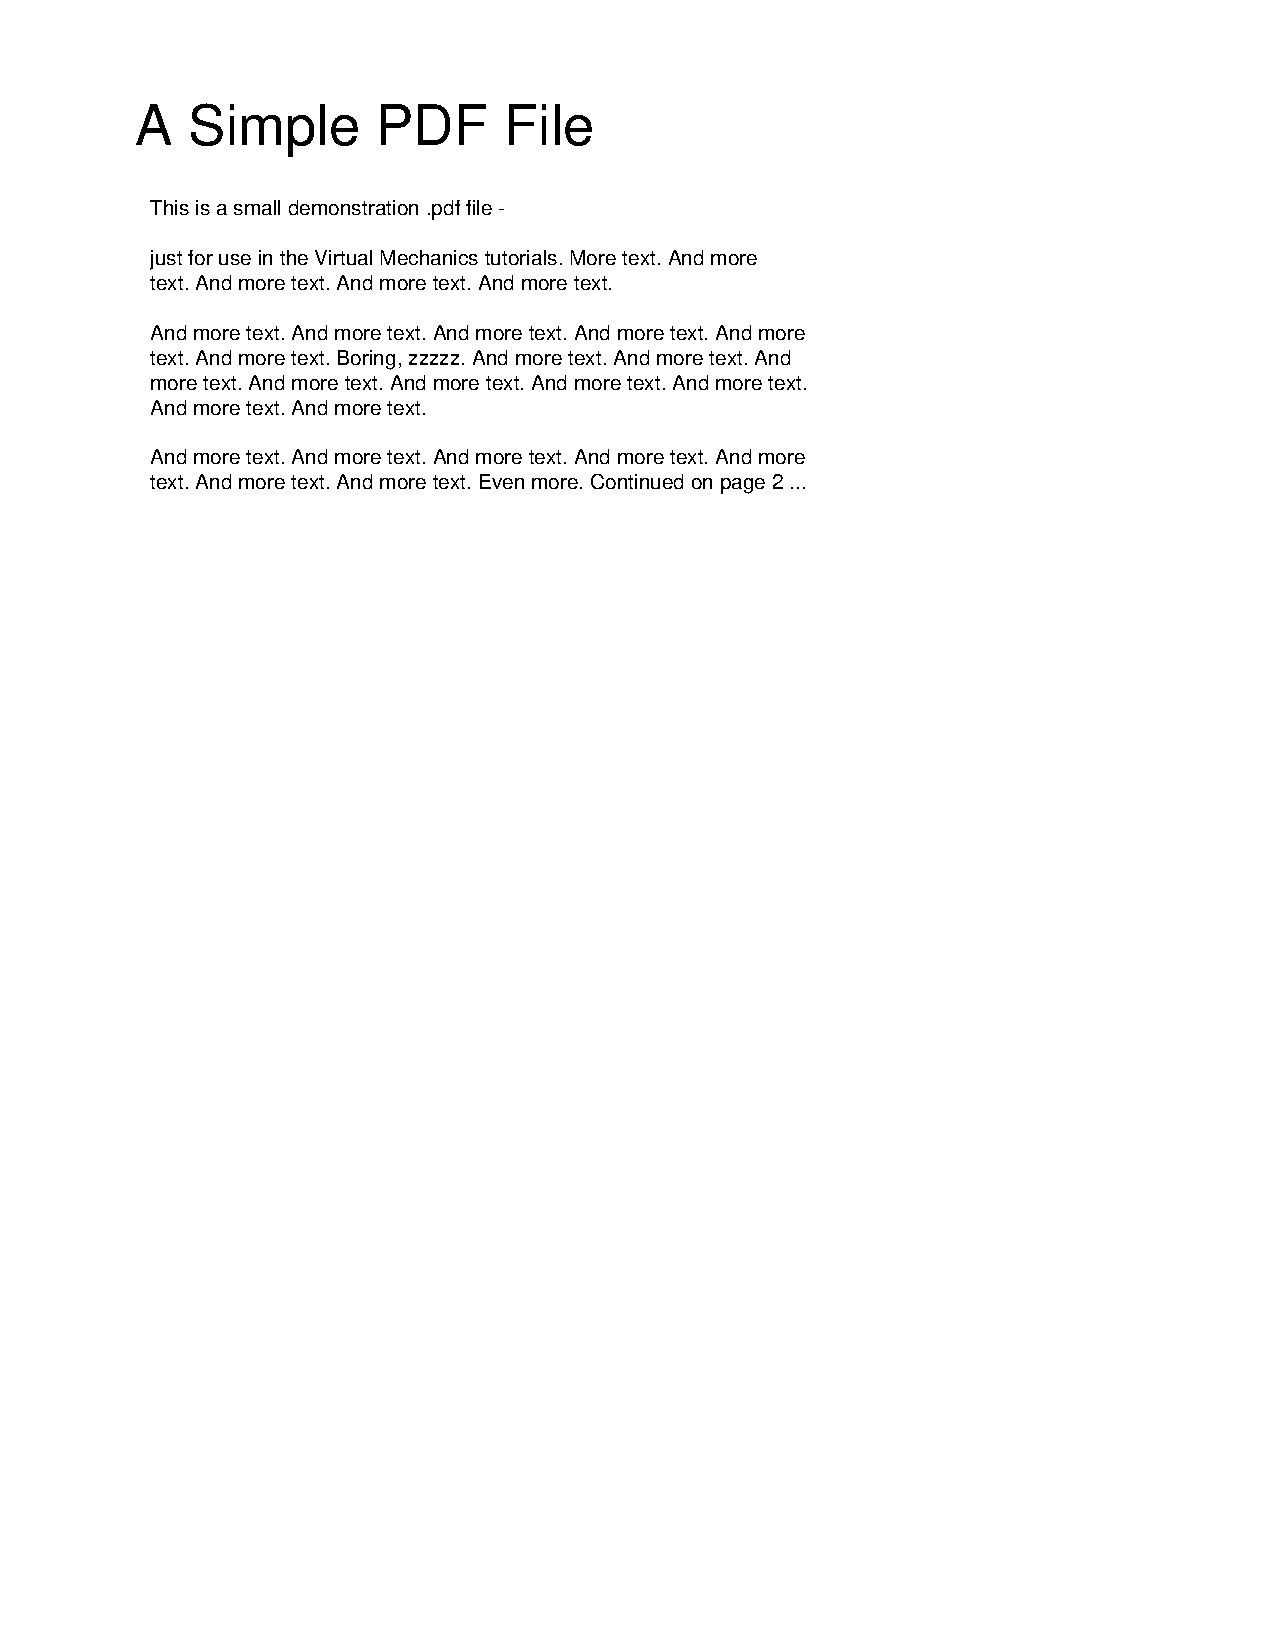
\includepdf[page=-]{Appendices/sample}

\paragraph{Sample PDF Only Page no.2} Only include the second page of a PDF file.It will start on next page and be inserted. 
% Format command : \includepdf[page={page number,page number,etc.}]{filename}
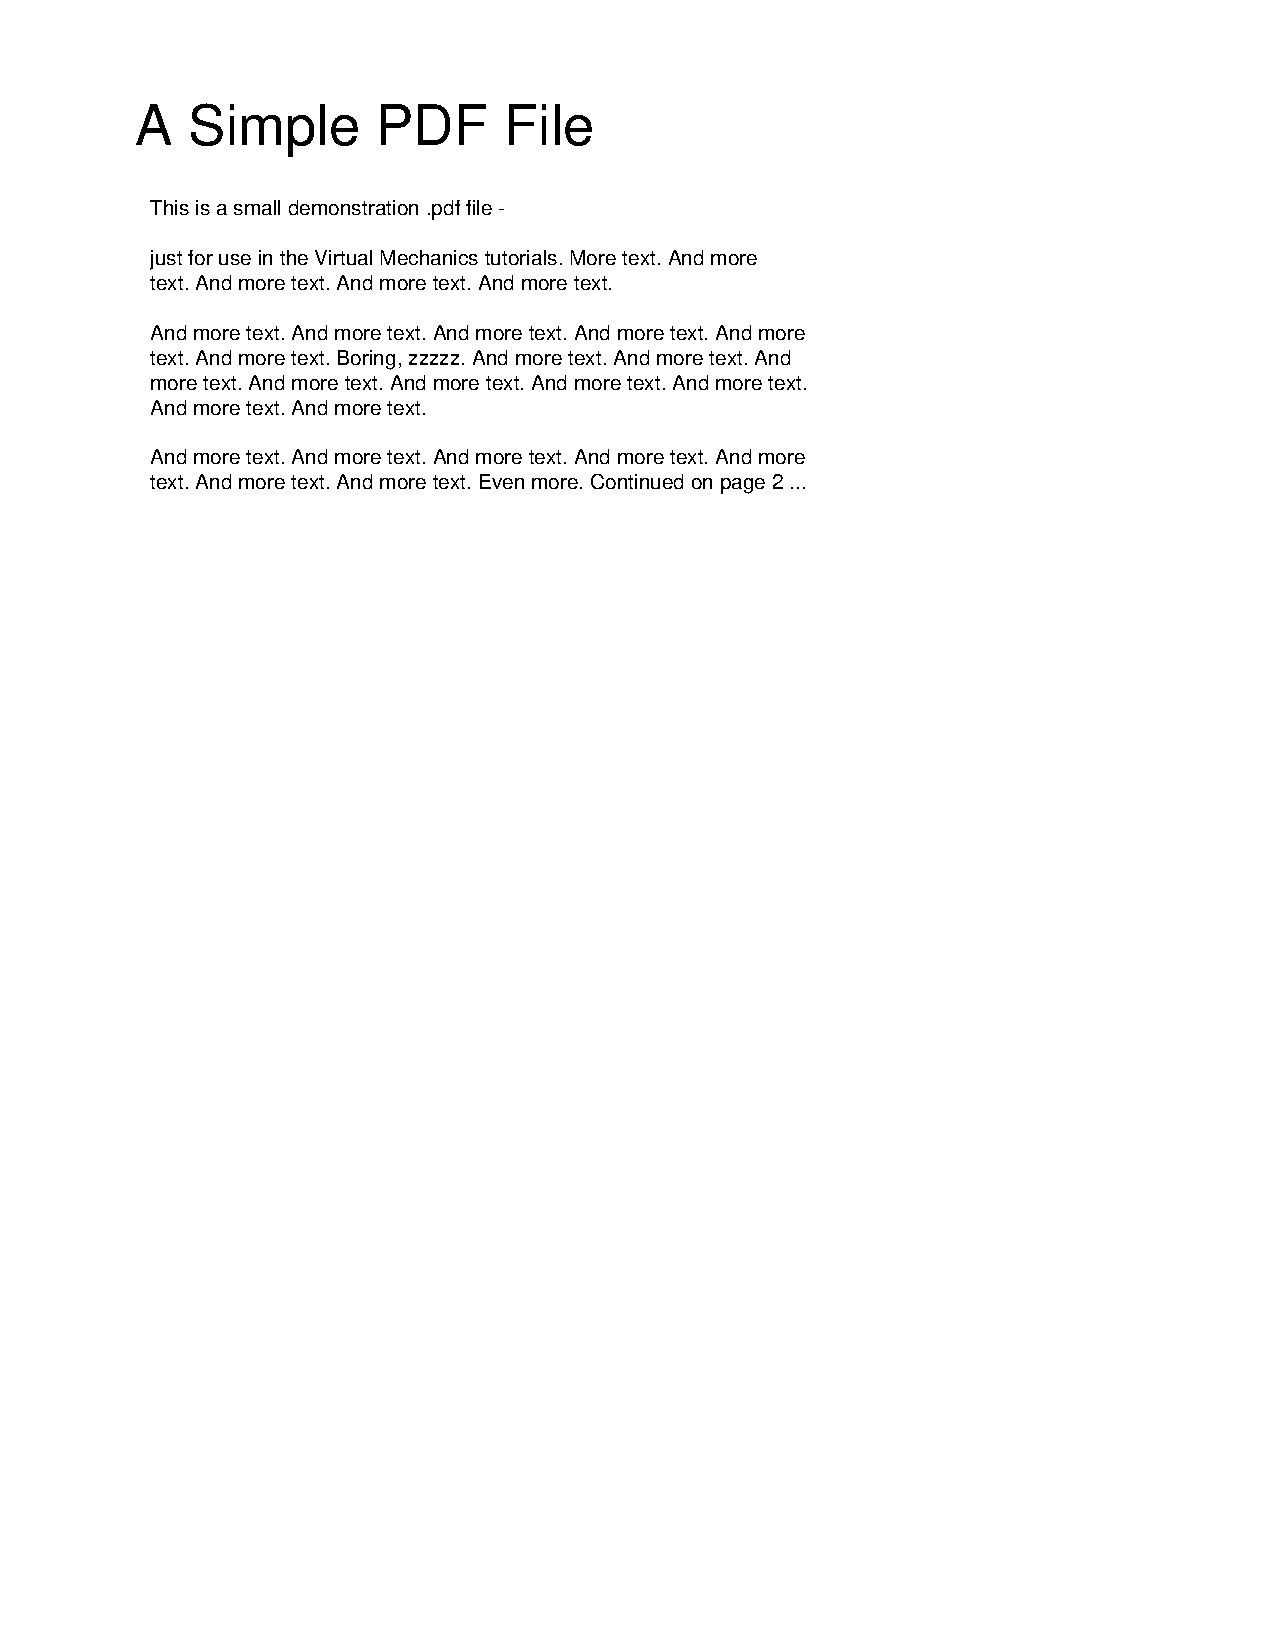
\includepdf[page={2}]{Appendices/sample}



\end{document}
